\subsection{GRASP-patterns}
\subsection{Design patterns}
\subsubsection{Composite}
\paragraph{}
We stellen onze constraints op onze emergency voor als een boom, deze implementatie is een toepassing van het \textit{Composite}-pattern, hierbij zien we \texttt{Dispatch\-Units\-Constraint} in de rol van \texttt{Component} de \texttt{Number\-Dispatch\-Units\-Constraint} is \'e\'en van de eventueel later uitgebreide \texttt{Leaf}s. Tot slot zien we \texttt{And\-Dispatch\-Units\-Constraint} als de \texttt{Composite} klasse. Gegeven de specificaties in de opgave is dergelijke structuur misschien ``overkill''. We zijn echter makkelijk in staat om nieuwe types constraints toe te voegen, net als connectoren (zoals bijvoorbeeld een OR).
\subsubsection{State}
Hoewel we geen cancel-emergency use-case moesten implementeren. Participeren we op de creatie van nieuwe staten waarin een emergency zich kan bevinden. Anderzijds willen we de voordelen die een \verb+enum+ ons biedt niet verliezen. Daarom opteerden we voor een hybride structuur. Deze structuur behoudt in zekere zin de geest van het \textit{State}-pattern beschreven in het boek \cite{book:designpatterns}. In \verb#C++# zijn \verb+enum+s echter niet polymorf: het is een lijst van waarden die met een binaire waarde geassocieerd worden. In java kunnen elementen in een enumeratie in zekere zin als een singleton-subklasse van de enumeratie beschouwd worden (uiteraard gaat die vergelijking niet volledig op). Het gevolg is dat we ook methodes aan deze elementen kunnen toewijzen, en dus individueel anders kunnen implementeren. In ons model beschouwen we een toestandsdiagram zoal op figuur \ref{fig:stateDiagramEmergency}.
\newcommand{\classComponent}{\umlClass{DispatchUnitsConstraint}{
\hline
areValidDispatchUnits(units:List<Unit>, used:boolean[]):boolean
}}
\begin{figure}
\centering
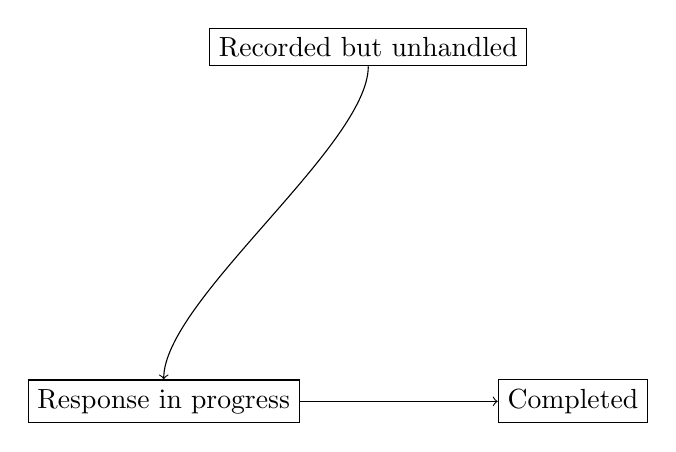
\begin{tikzpicture}
\node[rectangle,draw=black] (RBU) at (90:3) {Recorded but unhandled};
\node[rectangle,draw=black] (RIP) at (210:3) {Response in progress};
\node[rectangle,draw=black] (C) at (330:3) {Completed};
\draw[->] (RBU.south) .. controls +(down:10mm) and +(up:10mm) .. (RIP.north);
\draw[->] (RIP) -- (C);
\end{tikzpicture}
\caption{Beschrijving van de toestanden en overgangen van Emergency}
\label{fig:stateDiagramEmergency}
\end{figure}
